
The purpose of this chapter is to give an overview of the research areas
involved in this dissertation. First we explain the fundamental ideas of logic
programming and Prolog; next, the main concepts behind tabling evaluation are described,
focusing on the execution rules and strategies; finally, we introduce
the Yap and XSB Prolog systems, focusing on the tabling engines designed for both systems.

\section{Logic Programming}

Logic programming presents a declarative style of programming based on mathematical
logic and the predicate calculus. It is a very high level programming
paradigm that allows the programmer to focus on the problem at hand, leaving the
steps on \textit{how} to solve the problem to the computer.

In its purest form, logic programming is solely based on Horn Clause Logic \cite{Lloyd-87},
a subset of First Order Logic. Programming in logic can be viewed as
a two step process: (1) first, the theory is formulated as logic clauses,
next (2) we use this theory to search for alternative ways in which an arbitrary query is satisfied.

Logic programming is often mentioned to include the following advantages \cite{Carlsson-PhD}:

\begin{itemize}
  \item \textbf{Simple declarative semantics}: a logic program is simply a collection of predicate logic clauses.
  \item \textbf{Simple procedural semantics}: a logic program can be read as a collection of recursive procedures. In Prolog, for instance, clauses are tried in the order they are written and goals within a clause are executed from left to right.
  \item \textbf{High expressive power}: Logic programs can be seen as executable specifications that despite their simple procedural semantics allow for designing complex and efficient algorithms.
  \item \textbf{Inherent non-determinism}. Since in general several clauses can match a goal, problems involving search are easily programmed in these kind of languages.
\end{itemize}

\subsection{Logic Programs}

A logic program is composed by a set of Horn clauses. Each clause is a disjunction of literals
and contains at most one positive literal. Horn clauses are usually written as

\begin{center}
  $L_{1}, ..., L_{n} \Longrightarrow L  (\equiv \neg L_{1} \vee ... \neg L_{n} \vee L)$
\end{center}

or

\begin{center}
  $L_{1}, ..., L_{n}  (\equiv \neg L_{1} \vee ... \neg L_{n})$
\end{center}

where $n >= 0$ and $L$ is the only positive literal. 

A Horn clause that has exactly one positive literal is called a definitive clause; in the Prolog language
it is usually called a \textit{rule}.
A Horn clause without a positive literal is called a \textit{goal}.

Using Prolog's notation, one can write \textit{rules} in the form

\begin{center}
  $L :- L_{1}, ..., L{n}.$
\end{center}

Usually, $L$ is called the \textit{head} of the \textit{rule} and $L_{1}, ..., L_{n}$
the \textit{body} of the \textit{rule}, where each $L_{i}$ is called a subgoal.
A logical \textit{fact} is a special \textit{rule} where the \textit{body} is replaced by the \textit{true} symbol:

\begin{center}
  $L.$
\end{center}

Goals are \textit{rules} without the \textit{head} component and are also named as \textit{queries}.


Each literal in a Horn clause has the form $f(t_{1}, ..., t_{n})$, where $f$ is the \textit{functor} symbol
and each $t_{i}$ are \textit{terms}. A term can be a \textit{constant} (or \textit{atom}), a \textit{variable}
or a \textit{compound} term. Compound terms follow the functor structure, recursively.
Variables are assumed to be universally quantified and have the following major characteristics:

\begin{itemize}
  \item Variables are logical variables that can instantiated only once.
  \item Variables are untyped until instantiated.
  \item Variables are instantiated via \textit{unification}, a pattern matching operation that finds the most general common instance of two data objects. 
\end{itemize}

A sequence of clauses with the same functor in the head form a \textit{predicate}. The ordering
of these clauses can have some implications depending on the resolution semantics of the underlying language.
Prolog for instance, uses a top-down resolution mechanism known as \textit{SLD} (Selective Linear Definite) resolution \cite{Lloyd-87}.

SLD starts by matching the first subgoal query to the first clause of the respective predicate,
generating a new query using the body of the clause, which is added to the remaining query subgoals.
During this process a finite set of pairs $\theta$ called \textit{substitution} is built.
Each pair has the form $X = t$, where $X$ is a variable and $t$ is a term. No variable in the left-hand side
of a pair appears on the right-hand side and no two pairs have the same variable as left-hand side \cite{Sterling-94}. 
When the clause body is reused as query, all the variables present in the terms are replaced using the
set $\theta$. 
If unification fails, the next clause of the predicate is tried, using a mechanism called \textit{backtracking}.
This recursive computation fails when there are any more clauses left to try. It succeeds when the subgoal query is empty.

The resolution process is fundamentally non-deterministic and can be viewed as a search within a tree. SLD
does not force any specific search strategy for exploring the tree. Prolog for example, uses a depth-first, one
branch at a time search.

\subsection{Prolog and the WAM}
  
Prolog is one of the first logic programming languages and arguably the most successful.
The first implementation of Prolog was Marseille Prolog, developed in 1972 by Alain Colmerauer and Robert Kowalski \cite{Kowalski-74}.

The use of Prolog as a practical and efficient language was made viable by David Warren in 1977, when he built a compiler that could
compete with other languages like Lisp \cite{Warren-77}. Then in 1983, David Warren formulated an abstract machine known as WAM
(\textit{Warren Abstract Machine}) \cite{Warren-83} that is still widely used in modern Prolog implementations.

\subsubsection{Prolog}

Prolog follows the semantics of the SLD resolution through a depth first search strategy.
It starts by choosing the top-most clauses of the predicate and the subgoals are solved
within a left-to-right fashion.

\begin{figure}[ht]
\begin{verbatim}
factorial(0,1) :- !.
factorial(N,R) :-
  N > 0,
  N1 is N - 1,
  factorial(N1,R1),
  R is N * R1.
\end{verbatim}
\caption{Factorial function in Prolog.}
\label{fig:factorial_prolog}
\end{figure}

For illustration purposes, in Figure~\ref{fig:factorial_prolog} we define the predicate \texttt{factorial/2} that
computes the factorial of a given number. This predicate has arity of 2, where the first argument is an
\textit{input} argument and the second argument an \textit{output} argument.
Factorial is composed of two clauses, the first represents the factorial base case (factorial of 0 is 1) and
the second represents the recursive relation. The second clause first checks if the input number
is positive, to discard non-positive numbers, then computes $N - 1$ and recursively
calls factorial to compute the value of $factorial(N-1)$. Finally, the output argument $R$ is then unified
to $N * factorial(N-1)$. The first clause uses the \textit{cut} operator (\texttt{!})
that tells the Prolog engine to not explore alternative clauses, i.e., the factorial of 0 is not to be
computed using the recursive call defined on the second clause.
Once Prolog finds the first answer (Figure~\ref{fig:factorial_tree}), the cut control operator disables further
alternatives, completing the depth first search in the tree.

\begin{figure}[ht]
  \centering
    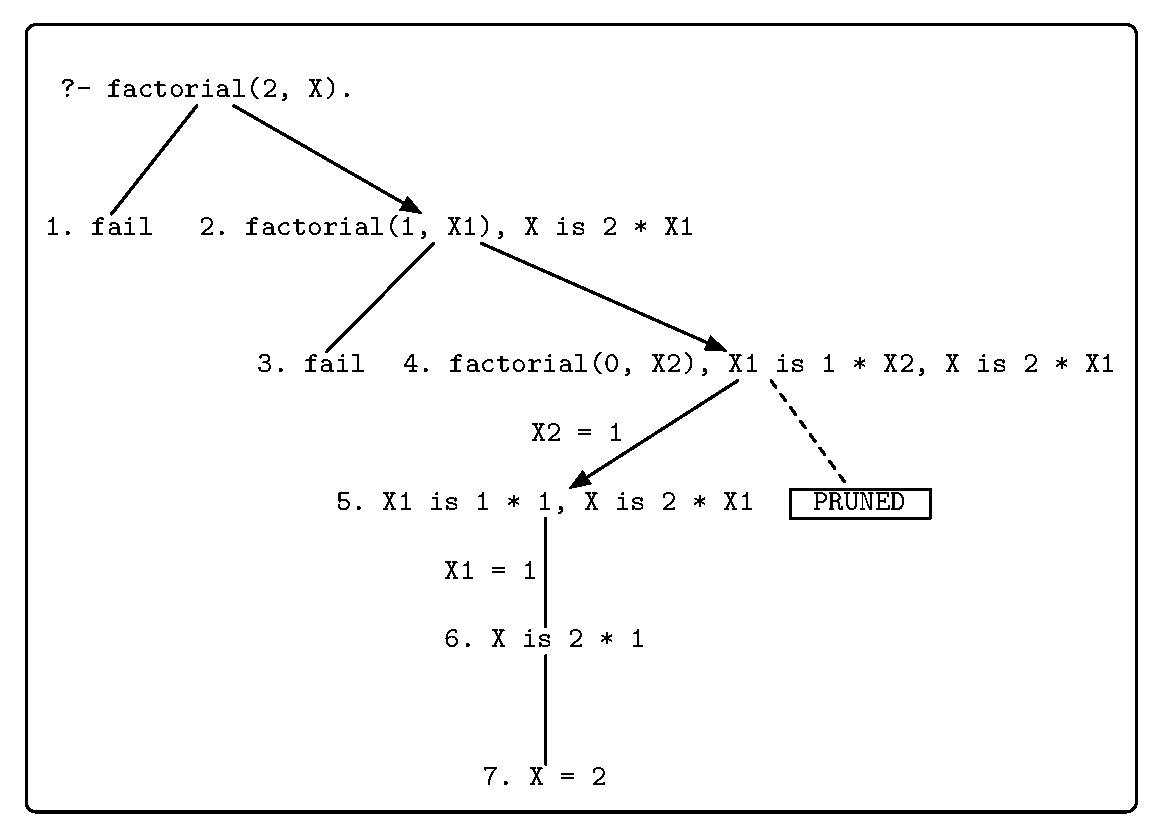
\includegraphics[scale=0.6]{factorial.pdf}
  \caption{Factorial search tree.}
  \label{fig:factorial_tree}
\end{figure}

The cut operator is not the only special instruction in Prolog, more built-in predicates are also available:

\begin{itemize}
  \item \textbf{Meta-logical predicates}: inquire the state of the computation and manipulate terms.
  \item \textbf{Extra-logical predicates}: manipulate the Prolog database, adding or removing clauses from
  the program being executed. Input/Output operators are another example of extra-logical predicates.
  \item \textbf{Other predicates}: predicates to perform arithmetic operations, to compare terms, to support debugging, etc.
\end{itemize}

These special operators make programming more practical and useful in real world applications.

\subsubsection{WAM}

The \textit{Warren Abstract Machine} (WAM) is a stack-based architecture
with various data areas, registers, and low level instructions that can be efficiently executed, manipulated and optimized.
A simplified layout is presented in Figure~\ref{fig:wam}.

\begin{samepage}
   
In terms of execution stacks, the WAM defines the following:

\begin{itemize}
  \item \textbf{PDL}: a push down list used by the unification process.
  \item \textbf{Trail}: stores the addresses of the variables that must be reset when backtracking.
  \item \textbf{Stack}: stores \textit{environment} and \textit{choice point} frames.
         Environments track the flow control in a program and consist of: the stack address of the
         previous environment; a pointer to the next instruction to execute upon return of the invoked
         clause; and a set of \textit{permanent variables} \footnote{A permanent variable is a variable
         which occurs in multiple body subgoals and must be preserved between calls.} as a sequence of cells.
         
         Choice points store open alternatives which are used to restore the state of the computation
         when backtracking. A pointer to the instruction for the next alternative is stored in case
         the current execution branch fails.
         A choice point is created when there are more than one alternative for a subgoal call.
         We pop the choice point from the stack when the last alternative clause is attempted. 
  \item \textbf{Heap}: array of data cells used to store variables and compound terms that cannot
         be stored in the stack.
  \item \textbf{Code Area}: contains the compiled instructions.
\end{itemize}

\end{samepage}

\begin{figure}[ht]
  \centering
    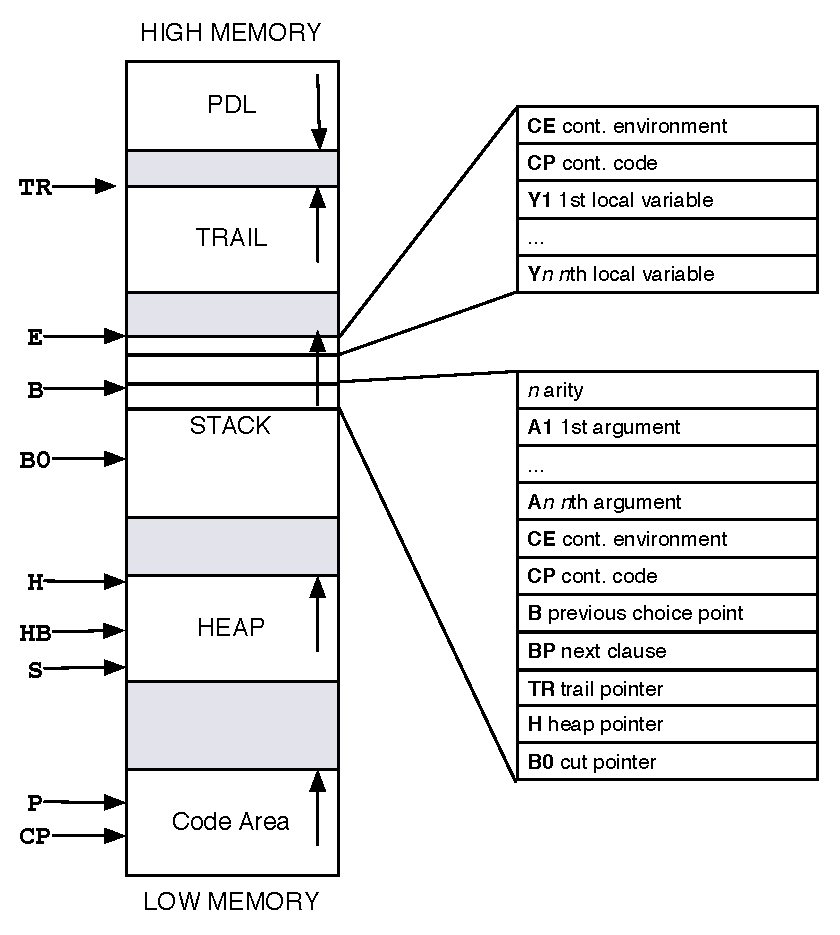
\includegraphics[scale=0.7]{wam.pdf}
  \caption{WAM memory layout, frames and registers.}
  \label{fig:wam}
\end{figure}

For the registers, WAM defines the following:

\begin{itemize}
  \item \textbf{P}: points to the current WAM instruction.
  \item \textbf{CP}: stores the value of \textbf{P} before the current invoked call and it is used to restore the execution point.
  \item \textbf{TR}: points to the top of the trail stack.
  \item \textbf{E}: points to the current active environment.
  \item \textbf{B}: the active choice point.
  \item \textbf{B0}: the choice point to return to upon backtracking over a cut.
  \item \textbf{H}: points to the top of the heap stack
  \item \textbf{HB}: marks the value of the register \textbf{H} at the time of the latest choice point. It is used to
  determine \textit{conditional} variable bindings that affect variables existing before the creation of the choice point.
  \item \textbf{S}: used during the unification of compound terms.
\end{itemize}

WAM instructions can be grouped into four main groups: choice point instructions to manipulate choice points; control
instructions to manage environments and control the execution flow; unification instructions that implement
specialized versions of the unification algorithm; and indexing instructions to efficiently determine which clauses
unify with a given subgoal call.

The WAM being a complex topic has complete books dedicated to explaining its intricacies.
An example is the \textit{Warren's Abstract Machine -- A Tutorial Reconstruction} written by H. A\"{\i}t-Kaci \cite{Aitkaci-91}. 

\section{Tabling}

Despite Prolog's declarativeness and expressiveness, the past few years have seen wide efforts at
solving shortcomings that arise when using SLD resolution.
One proposal that has gained popularity is \textit{tabling} or \textit{tabulation} \cite{Chen-96}.
In comparison to the traditional SLD resolution method, tabling can reduce the search space to cut redundant computations,
avoids looping and has better termination properties \cite{Tamaki-86}.

In a nutshell, tabling is a refinement of the SLD resolution that consists in storing intermediate answers for
subgoals so that they can be reused when a repeated subgoal appears in the resolution process.
The use of tabling enables the programmer to write more expressive, but still valid, logical programs.

\begin{figure}[ht]
\begin{verbatim}
:- table path/2.

path(X,Z) :- edge(X,Y), path(Y,Z).
path(X,Z) :- edge(X,Z).

edge(a,b).
edge(b,a).
\end{verbatim}
\caption{The \texttt{path} program.}
\label{fig:prolog_path}
\end{figure}

One classical example that is used to demonstrate the advantages of using tabling is presented in Figure~\ref{fig:prolog_path}.
This program describes the predicate \texttt{path/2} that computes reachability between two nodes on a directed graph.
Connections are established as facts using the \texttt{edge/2} predicate.
If we tried to evaluate the query goal \texttt{path(X,Z)}, traditional Prolog would enter an infinite
loop (Figure~\ref{fig:infinite_loop}) because \texttt{edge/2} facts define a cyclic graph and the first
clause of \texttt{path/2} is right recursive, leading to a repeated call.

\begin{figure}[ht]
  \centering
    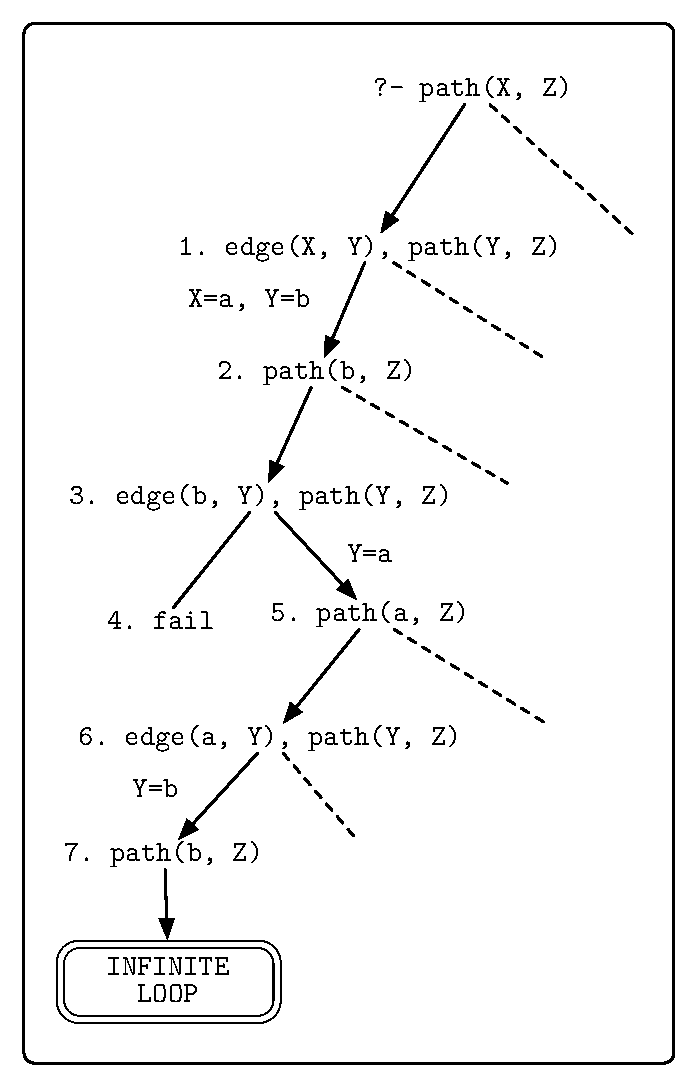
\includegraphics[scale=0.6]{infinite_loop.pdf}
  \caption{Infinite loop evaluating \texttt{path(X, Z)}.}
  \label{fig:infinite_loop}
\end{figure}

\subsection{Tabled Evaluation}

In this new method of evaluation, when a tabled subgoal is first called, a new entry is allocated on the \textit{table space}. Table
entries are used to store subgoal calls but they also store answers found during evaluation. Each time a tabled subgoal is called, we
know if it is a repeated call by inspecting the table space. Nodes in the search space can thus be classified as:
\textit{generator nodes}, if they are being called for the first time; \textit{consumer nodes} if they are repeated calls;
or \textit{interior nodes} if they are non-tabled subgoals. Generator nodes are matched against the predicate clauses as usual but
consumer nodes are not, instead they consume answers stored in the table space from the respective subgoal.

In Figure~\ref{fig:tabling_path} we depict the tabled evaluation of the query goal \texttt{path(X,Z)}.
Generator nodes are represented by rectangles with double lines and consumer nodes by simple rectangles.
Note that we need to declare \texttt{path/2} as tabled using the \texttt{table} directive.

Tabled evaluation starts by inserting a new entry in the table space and by allocating a generator
node to represent \texttt{path(X,Z)} (step 1). Like SLD resolution, \texttt{path(X,Z)} is then resolved
against the first \texttt{path/2} clause (step 2). The goal \texttt{edge(X,Y)} is not tabled and is
resolved as usual. We use the first \texttt{edge/2} clause with \texttt{\{X~=~a,~Y~=~b\}} and these values
are carried to \texttt{path(b,Z)} (step 3). This goal is not yet in the table space, hence we add a new entry for it.

Goal \texttt{path(b,Z)} is then resolved against the first clause of \texttt{path/2} (step 4).
Ñext, \texttt{edge(b,Y)} fails against the first clause but succeeds with \texttt{\{Y~=~a\}} for
the second clause. A new tabled subgoal \texttt{path(a,Z)} is registered in the tabled space (step 6)
and resolved against the first clause of \texttt{path/2} (step 7). This time the \texttt{edge/2}
subgoal matches with the first clause with \texttt{\{Y = b\}}. This originates a repeated tabled subgoal
call to \texttt{path(b,Z)} and the first consumer node is allocated (step 8). As we have no answers for \texttt{path(b,Z)}
in the table space, the current evaluation point is \textit{suspended}. Later on, this node can be resumed to
consume new answers.

Next, we backtrack to node 7 and try the second \texttt{edge/2} clause, but resolution fails (step 9). We backtrack again, this time to
node 6 to try the second clause of \texttt{path/2} (step 10). Here \texttt{edge(a, Z)} is resolved against the
first clause of \texttt{edge/2} and the answer \texttt{\{Z~=~b\}} is found for the subgoal \texttt{path(a,Z)} (step 11).
This answer is stored in the table space and forward execution is made, propagating the binding \texttt{\{Z~=~b\}} to
\texttt{path(b,Z)}, and a first answer to this subgoal is also found and stored in the table space (step 12).
We continue forward execution and the binding is once again propagated, this time to node 3 finding an answer to
\texttt{path(X,Z)} and to the query subgoal, \texttt{\{X~=~a,~Z~=~b\}} (step 13).

\begin{figure}[ht]
  \centering
    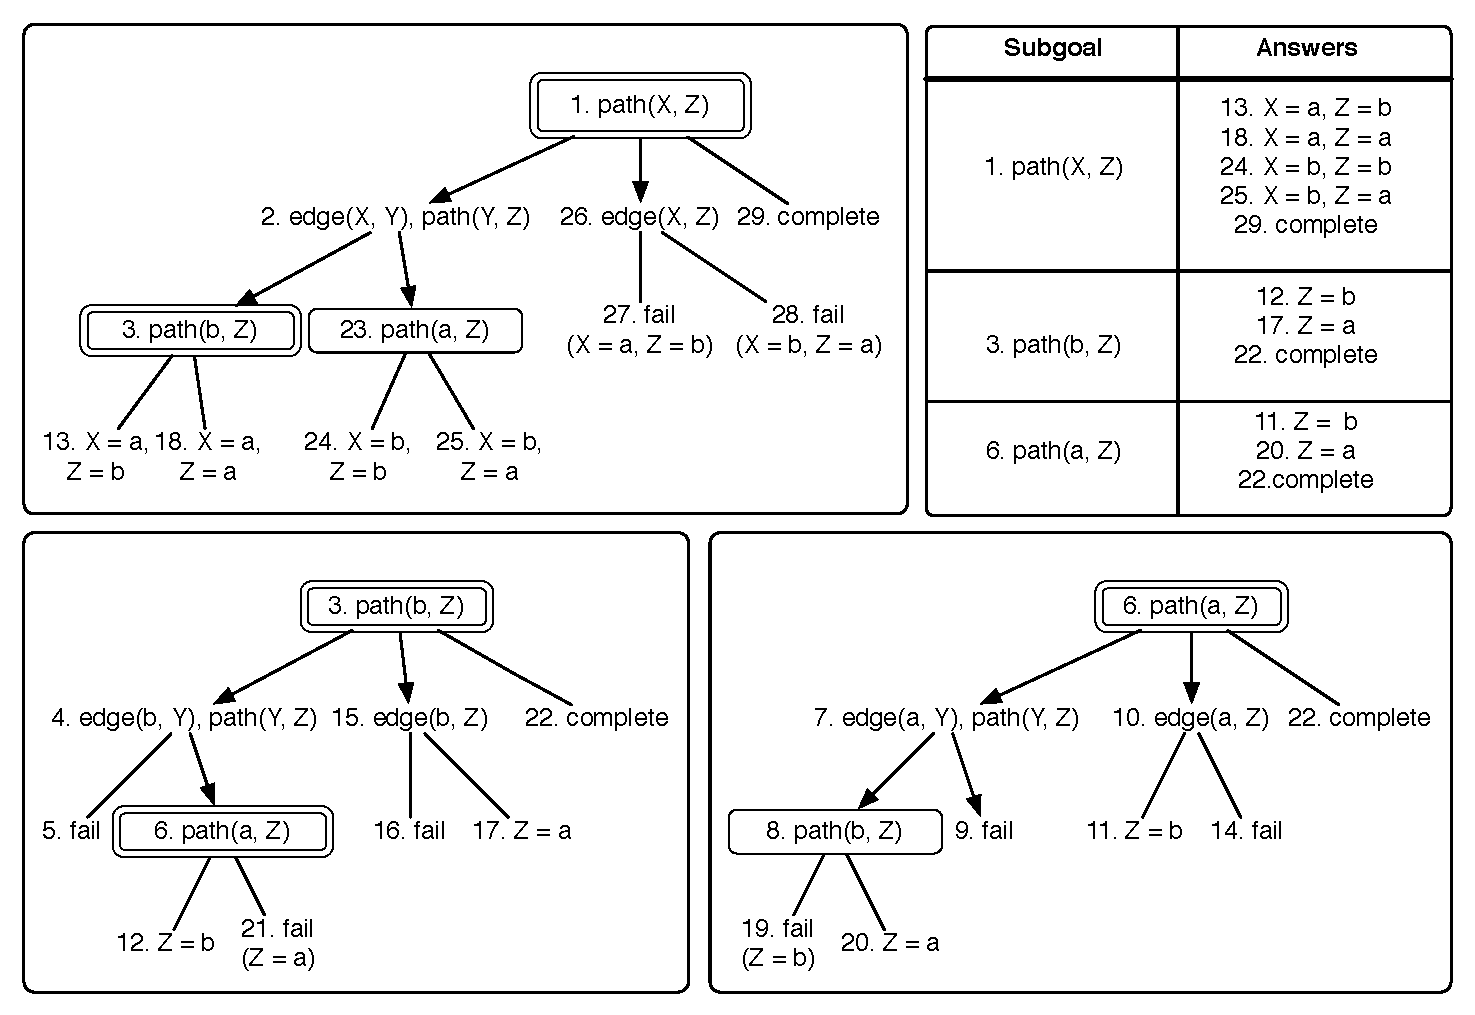
\includegraphics[scale=0.6]{tabling_path.pdf}
  \caption{Tabled evaluation of \texttt{path(X,Z)}.}
  \label{fig:tabling_path}
\end{figure}

If the user asks for more answers, the computation returns to node 10 to try the second clause of
\texttt{edge/2}, but it fails (step 14). The process backtracks to node 6 but at this node there
are no more clauses left to try. Moreover, we can not complete the subgoal \texttt{path(a,Z)} because
it depends on a older subgoal (node 3 is the generator node for the consumer node 8 under it), thus we backtrack to node 3.

At node 3, the second clause of \texttt{path/2} is tried (step 15) and the first clause of
\texttt{edge/2} fails (step 16), but the second succeeds with a new answer for \texttt{path(b,Z)},
\texttt{\{Z~=~a\}} (step 17). Again, we propagate variable bindings in step 18, generating a new
answer to subgoal \texttt{path(X,Z)}, \texttt{\{X~=~a,~Z~=~a\}}.

We go back to node 3, where no more clauses are available, but now completion can be safely
attempted because all consumers in lower branches do not depend on any generator node older
than node 3. Node 3 is called, by definition, a \textit{leader node} and the branch of nodes
below it form a \textit{Strongly Connected Component} (SCC) \cite{Tarjan-72}.

However, by inspecting the execution tree, we can see that node 8 has two unconsumed answers.
We thus resume the computation at node 8 to consume the answer \texttt{\{Z~=~b\}} and forward it to subgoal
\texttt{path(a,Z)} at node 6 (step 19). Here, we note that it is a repeated answer
to this subgoal by checking the table space, and thus we fail (step 19).
Failing repeated answers is crucial to avoid unnecessary computations and sometimes looping.

Then, we fetch the next available answer, \texttt{\{Z~=~a\}}, that is propagated
to node 6, generating a new answer to \texttt{path(a,Z)} (step 20). This binding
is once again propagated, now for node 3 but it is a repeated answer, and thus
the computation fails (step 21). With no more unconsumed answers, we
return back to node 3 to re-attempt completion. This time, no consumers have
unconsumed answers and we can safely complete all the subgoals in the current SCC
(step 22). Subgoals \texttt{path(b,Z)} (node 3) and \texttt{path(a,Z)} (node 6)
are marked as \textbf{complete} in the table space and no new answers are accepted.

Next, we backtrack to node 2 to try the second \texttt{edge/2} clause. A new consumer node is allocated (step 23) and answers can be
promptly consumed from the table space as the subgoal \texttt{path(a,Z)} is already completed.
The retrieved answers in step 23 are propagated to node 1 and new answers are generated (steps 24 and 25).

We backtrack to node 1 to try the second \texttt{path/2} clause (step 26). Resolution succeeds for both
\texttt{edge/2} clauses but as the newly found answers
are repeated we fail for both cases (steps 27 and 28). The process backtracks again to node 1 and with no more clauses to try,
we attempt completion. As there are no consumer nodes, completion is done (step 29) and computation terminates successfully.

From the described example we can summarize four main operations needed to support tabled evaluation:

\begin{itemize}
  \item The \textit{tabled subgoal call} operation represents a call to a tabled subgoal.
  If the subgoal is already in the table space, it creates a new consumer node to consume answers.
  If it is a new subgoal call it creates a new generator node and adds a new entry to the table space.
  Each new entry is initialized with an empty set $S$ that will contain the answers for the subgoal. 
  
  \item The \textit{new answer} operation adds a new answer $s$ to the table space. If the answer is repeated the operation fails,
  otherwise a new answer set $S'$ for the subgoal is generated: $S' \equiv S \cup {s}$.
  
  \item The \textit{answer resolution} operation checks wether new answers from the table space are available for consumption.
  When no new answers are available, the consumer node is \textit{suspended} and execution proceeds using a specific strategy.
  Given the last consumed answer, we determine the unconsumed answer
  set $R$ ($R \subseteq S$) and fetch the element $r \in R$, which is the first element from the set $R$. The last consumed answer
  can be seen as a \textit{continuation} that is stored in each consumer node and is used to determine the next available answer.
  
  \item The \textit{completion} operation determines if a tabled subgoal is \textit{completely evaluated}.
  Only leader nodes can complete themselves and younger generator nodes.
  Once a subgoal is completed the set of answers $S$ is closed and no more answers are accepted; future subgoal calls
  can use the set $S$ without the need to suspend.
\end{itemize}

\subsection{Tabling Instructions}

Tabling engines extend the WAM instruction set with \textit{tabling instructions} to support the four
main tabling operations. Usually, each tabled predicate is compiled by using
variants of the following instructions:
\texttt{table\_try}, \texttt{table\_retry} and \texttt{table\_trust}. These instructions
are very similar to \texttt{try\_me}, \texttt{retry\_me} and
\texttt{trust\_me}, which the WAM natively implements. 

For tabled predicates with multiple clauses, \texttt{table\_try} is used on the first clause,
\texttt{table\_retry} for the middle clauses and \texttt{table\_trust} for the last clause.
Predicates with a single clause use a special instruction: \texttt{table\_try\_single}.

\begin{figure}[ht]
\begin{Verbatim}
path/2_1:
  table_try_me path/2_2
  % WAM code for path(X,Z) :- edge(X,Y), path(Y,Z).
  new_answer
path/2_2:
  table_trust_me
  % WAM code for path(X,Z) :- edge(X,Z).
  new_answer
\end{Verbatim}
\caption{Compiled code for the tabled predicate \texttt{path/2}.}
\label{fig:compiled_tabled_path}
\end{figure}

The \texttt{table\_try} instruction implements the tabled subgoal call operation. If the subgoal is called
for the first time, the data structures associated with this subgoal and a new generator node are created.
Execution then proceeds by executing each predicate clause. This is performed by the \texttt{table\_retry}
instruction, which alters the next instruction of the generator choice point to the next clause of the predicate.
On the other hand, if the subgoal is repeated, a consumer choice point is allocated and set to execute the
\texttt{answer\_resolution} instruction, which consumes answers and implements the answer resolution operation.

The instruction \texttt{table\_trust} is executed by generator nodes and sets the next
instruction to execute upon backtracking to
\texttt{completion}, which runs the completion operation.

Finally, at the end of each clause, the instruction \texttt{new\_answer} is appended to implement
the new answer operation. This instruction has access to the arguments of a tabled subgoal call,
thus by dereferencing them it obtains the corresponding answer, which can be added into the table space.    

\subsection{Scheduling Strategies}

During evaluation of the previous example it is very clear that at several points we can choose between
different \textit{scheduling} strategies: continue forward execution, backtrack to interior nodes,
return answers to consumer nodes, or perform completion. Depending on how and when the return of answers
is scheduled, different strategies and searches can be formulated. It is also well known that using
different strategies can lead to tremendous effect on performance as some predicates are better suited to specific strategies. 
The most popular scheduling strategies are \textit{batched scheduling} and \textit{local scheduling} \cite{Freire-96}.

Batched scheduling reduces the need to suspend and move around the search tree by batching the return of answers.
When the engine generates answers, while evaluating a particular goal, the answers are added to the table and
the subgoal continues its normal evaluation until it resolves all available program clauses. Only then the answers
are consumed by consumer nodes \cite{Freire-96}. In some cases, this results in creating dependencies to older
subgoals, therefore enlarging the current SCC and delaying completion to older generator nodes. When backtracking,
three situations may arise:

\begin{itemize}
  \item if backtracking to a generator or interior node, try the next available clause.
  \item if backtracking to a consumer node, consume new answers.
  \item if no more clauses are left to try or no more unconsumed answers are available, two new situations may arise:
    \begin{itemize}
      \item if the node is a leader node, attempt completion.
      \item if not, backtrack to a previous branch.
    \end{itemize}
\end{itemize}

Note that batched scheduling was the strategy used in the evaluation of the example in Figure~\ref{fig:tabling_path}.

For some problems, local scheduling is better suited because it tries to evaluate a single exact SCC at a time, preserving the dynamic
SCC ordering during the evaluation. In other words, in a local evaluation, answers are returned to consuming nodes outside of an SCC only after that
SCC is completely evaluated \cite{Freire-96}.
It differs from batched scheduling in that once the answers are found, they are added to the table space, but execution
\textit{fails}. Because this strategy tries to complete sooner rather than later, we can expect less dependencies between subgoals.

\subsection{Variant Tabling} \label{sec:variant_tabling}

When the subgoal \texttt{path(X,Z)} is called, a check for the presence of this subgoal in the table space is done first.
In the example in Figure~\ref{fig:tabling_path}, this was done by checking wether a \textit{variant} of the new goal already
exists in the table. We say that two terms $t_1$ and $t_2$ are variants of each other if they are identical up to renaming of their
variables.

For example, \texttt{path(X,Z)} is variant of the subgoal \texttt{path(X,Y)}, as they represent the same subgoal if we try
to rename their variables to a standardized format. One format was proposed by Bachmair \textit{et al} \cite{Bachmair-93}. Formally,
we have a set $V$ of variables present in a term and a function $renameVar$, such that the first term variable $v0 \in V$
results in $renameVar(v0) = VAR0$ and the following distinct variables are named incrementally ($VAR1, VAR2, ...$).
Using this mechanism, \texttt{path(X,Z)} and \texttt{path(X,Y)} both result in \texttt{path(VAR0,VAR1)}. The resulting
standardized subgoal is then checked against the table space to verify if it is a repeated subgoal call.

The variant approach is widely used in tabling systems, but other approaches do exist. One approach named
\textit{call by subsumption} works by checking wether the new goal is subsumed by another goal in the table space.
In other words, we verify if there is a more general subgoal than the one being called. For example
\texttt{path(b,Z)} is subsumed by the subgoal \texttt{path(X,Z)}.

In this approach, instead of creating
a new generator node at step 3, we create a consumer node that would consume answers stored in the subgoal \texttt{path(X,Z)}.
For correct results, it should be clear that the answers used from the table space must unify with \texttt{path(b,Z)}.
Like variant tabling, those new consumer nodes do not expand by using the program clauses, hence the search tree for this new
method will be greatly reduced. This new approach will be throughly explored in the next chapter.

  \subsection{Yap and XSB}
  
  Yap \cite{system-yap} and XSB \cite{system-xsb} are two well known Prolog systems that implement tabling.
  
  The YAP Prolog system is a high-performance Prolog compiler developed at the University of Porto.
  It is one of the fastest available Prolog systems and implements a wide range of functionalities: 
  stream I/O, sockets, modules, exceptions, debugging, a C-interface, dynamic code, internal database,
  DCGs, saved states, co-routining, arrays, threads and tabling.
  It is based on the WAM and follows the Edinburgh tradition. Most of the ISO-Prolog standard is implemented.
  
  Tabling in Yap is implemented through the YapTab sub-system \cite{Rocha-05a}, a suspension based tabling engine supporting evaluation of
  definite programs. YapTab follows the seminal SLG-WAM (Linear resolution with Selection function for General logic programs in WAM)
  design from XSB Prolog \cite{Sagonas-96, Sagonas-98},
  but it innovates by proposing a new fix-point check algorithm, and by considering that the control of fix-point detection should be
  performed at the level of the data structures corresponding to suspended sub-computations. YapTab was originally designed to achieve
  good results in sequential tabling, but could be extended with the OPTYap engine, for parallel execution \cite{Rocha-05a}.
  Other innovations in YapTab include: support for a dynamic combination of batched and local scheduling \cite{Rocha-05c}
  and efficient handling of \textit{incomplete tables} \cite{Rocha-06b}. Incomplete tables are created when the current computation is pruned from the execution stacks, keeping the pruned subgoals from retrieving
  the complete answer set. Currently, only call by variant checking is supported.
  
  XSB is a research-oriented logic programming system for Unix and Windows based systems. In addition to providing all
  the functionality of the Prolog language, XSB contains several features not usually found in logic programming systems,
  namely, evaluation according to the Well-Founded Semantics (tabling with negation) \cite{Gelder-91} through the use of
  a delaying-based tabling engine, the SLG-WAM.
  Other features of XSB include: a fully threaded engine, constraint handling for tabled programs on a engine level, a variety of indexing
  techniques, interfaces to other languages, various compiler directives like \texttt{auto\_table}, which does static
  analysis to decide which predicates to table, etc. \cite{system-xsb}.
  
  SLG-WAM supports both tabling by variant checking and by subsumption checking.
  Tabling by call-subsumption was initially implemented by a technique called
  \textit{Dynamic Threaded Sequential Automata} \cite{Rao-96} and is currently
  implemented using \textit{Time Stamped Tries} \cite{Johnson-99}.

  In terms of design, both YapTab and SLG-WAM introduce the following extensions to the traditional WAM machine:
  the table space; a new set of registers, the \textit{freeze registers}, one per stack (local stack, heap and trail);
  an extension of the standard trail,
  called the \textit{forward trail}; and the tabling operations: \textit{tabled subgoal call},
  \textit{new answer}, \textit{answer resolution}, and \textit{completion}.

  The set of freeze registers says where stacks are frozen and protect the space belonging to suspended
  computations until the completion of the appropriate SCC takes place. They need to be adjusted
  in two different situations: when a computation suspends, increasing the portion of frozen stacks; and when a completion takes place,
  releasing part of space previously frozen.

  The forward trail is used to restore all the variable bindings to their state at the time the computation was suspended.
  Thus, the WAM trail is extended with parent trail entry pointers to create this new trail.
  Also, a new register is created, the \textbf{TR\_FZ} trail freeze register.

  The differences between SLG-WAM and YapTab reside in the data structures and algorithms used to control the process of leader detection
  and the scheduling of unconsumed answers. These differences are described next in more detail.
  
  \subsubsection{SLG-WAM}

  The SLG-WAM considers that evaluation control should be done at the level of the data structures
  corresponding to first calls to tabled subgoals, and does so by associating \textit{completion frames}
  to generator nodes \cite{Sagonas-98}.

  The \textit{completion stack} maintains, for each subgoal $S$, a representation of the deepest subgoal
  $S_{dep}$ upon which $S$ or any subgoal on top of $S$ may depend.

  When $S$ and all subgoals on top of $S$ have exhausted all program and answer clause resolution,
  $S$ is checked for completion. If $S$ depends on no subgoals deeper than itself, $S$ and
  all subgoals on top of $S$ are completely evaluated. Otherwise, if $S_{dep}$ is deeper in the completion
  stack than $S$, $S$ may depend upon subgoals that appear below it in the completion stack, and cannot be completed \cite{Sagonas-98}.

  A one-to-one correspondence exist between completion stack frames and generator nodes, as the completion stack frame
  is pushed onto the stack when a new tabled subgoal is called. A completion frame is popped off when a subgoal is
  completed. Also, each subgoal frame contains a pointer to completion frame.

  Consumer and generator choice points are extended to support the suspend and resume mechanism.
  The generator choice contains the following extra data: an explicit pointer of the failure continuation to take
  upon backtracking out of the choice point; a cell that records the value of a new global register,
  called the \textbf{RS} (\textit{root subgoal register}) register,
  which points to the root subgoal of the node currently under execution;
  a pointer to the subgoal frame; a set of freeze registers, so that the stored values can be restored later on;
  and an area called the \textit{substitution factor}, the set of free variables which exist in the terms in the argument registers.

  The consumer choice point is extended with: a copy of the \textbf{RS} register; a pointer of the failure continuation to take
  upon backtracking; a substitution factor; the last consumed answer continuation; and a pointer to chain
  together all consumer choice points of the same subgoal. 

  \subsubsection{YapTab}

  In YapTab, it is considered that the control of leader detection and scheduling of unconsumed answers should be
  performed through the data structures corresponding to repeated calls to tabled subgoals, and it associates a new
  data structure, the \textit{dependency frame}, to consumer nodes \cite{Rocha-00a}. Each consumer choice point thus
  contains a field that points to the respective dependency frame.

  Dependency frames are used to check for completion points and to move across the consumer nodes with unconsumed answers,
  thus they are linked together, forming the \textit{dependency space}.

  Generator choice points are WAM choice points extended with the substitution factor area, a pointer
  to the subgoal frame and, a pointer to a dependency frame. This pointer
  is only used when local scheduling is employed. A generator node for local scheduling only exports its answers to the calling
  environment when all clauses for the subgoal have been exhausted, hence it must act like a consumer.

  In SLG-WAM, if we want to release space previously frozen and restore the freeze registers, we use the
  stack values stored in the generator choice point to perform completion. In YapTab, as the freeze registers
  are not saved there, we use the top stack values kept in the youngest consumer choice point younger than the current completion point.

  YapTab reduces the size of consumer choice points by using dependency frames. Each frame contains the
  following fields: \textbf{last\_answer} field that stores the last answer consumed by the choice point;
  the \textbf{cons\_cp} field that points to the consumer choice point; the \textbf{leader} field which
  points to the leader node at creation time; and the \textbf{back\_leader} field that changes during
  evaluation, pointing to the leader node where we performed the last unsuccessful completion operation.
  A new global register, called \textbf{TOP\_DF}, always points to the youngest dependency frame.
